\section{Introduction}

\begin{frame}{Why Statistics?! Data-driven Modeling Applications}
    \begin{figure}
        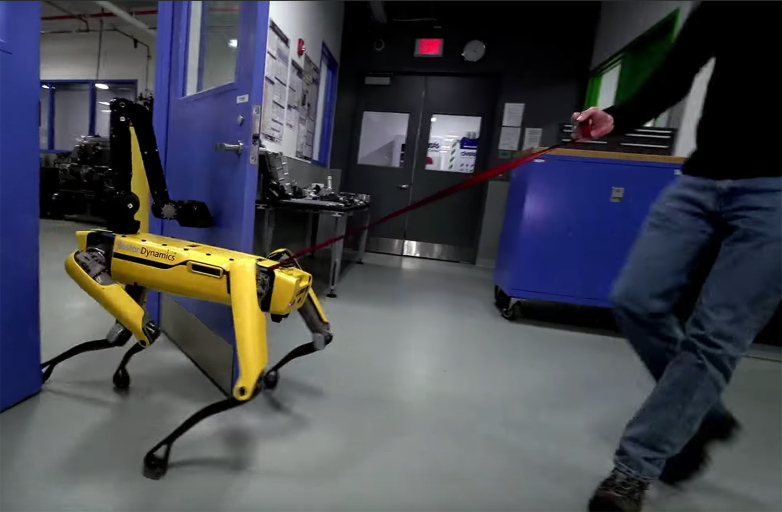
\includegraphics[width=0.9\textwidth]{gfx/web/boston-dynamics}\\
        SpotMini robot\\
        {\tiny Image: \href{https://www.bostondynamics.com/}{https://www.bostondynamics.com/}}
        {\tiny Movie: \url{https://www.youtube.com/watch?v=aFuA50H9uek}}
    \end{figure}

\end{frame}

\begin{frame}{Why Statistics?! Data-driven Modeling Applications}
    \begin{figure}
        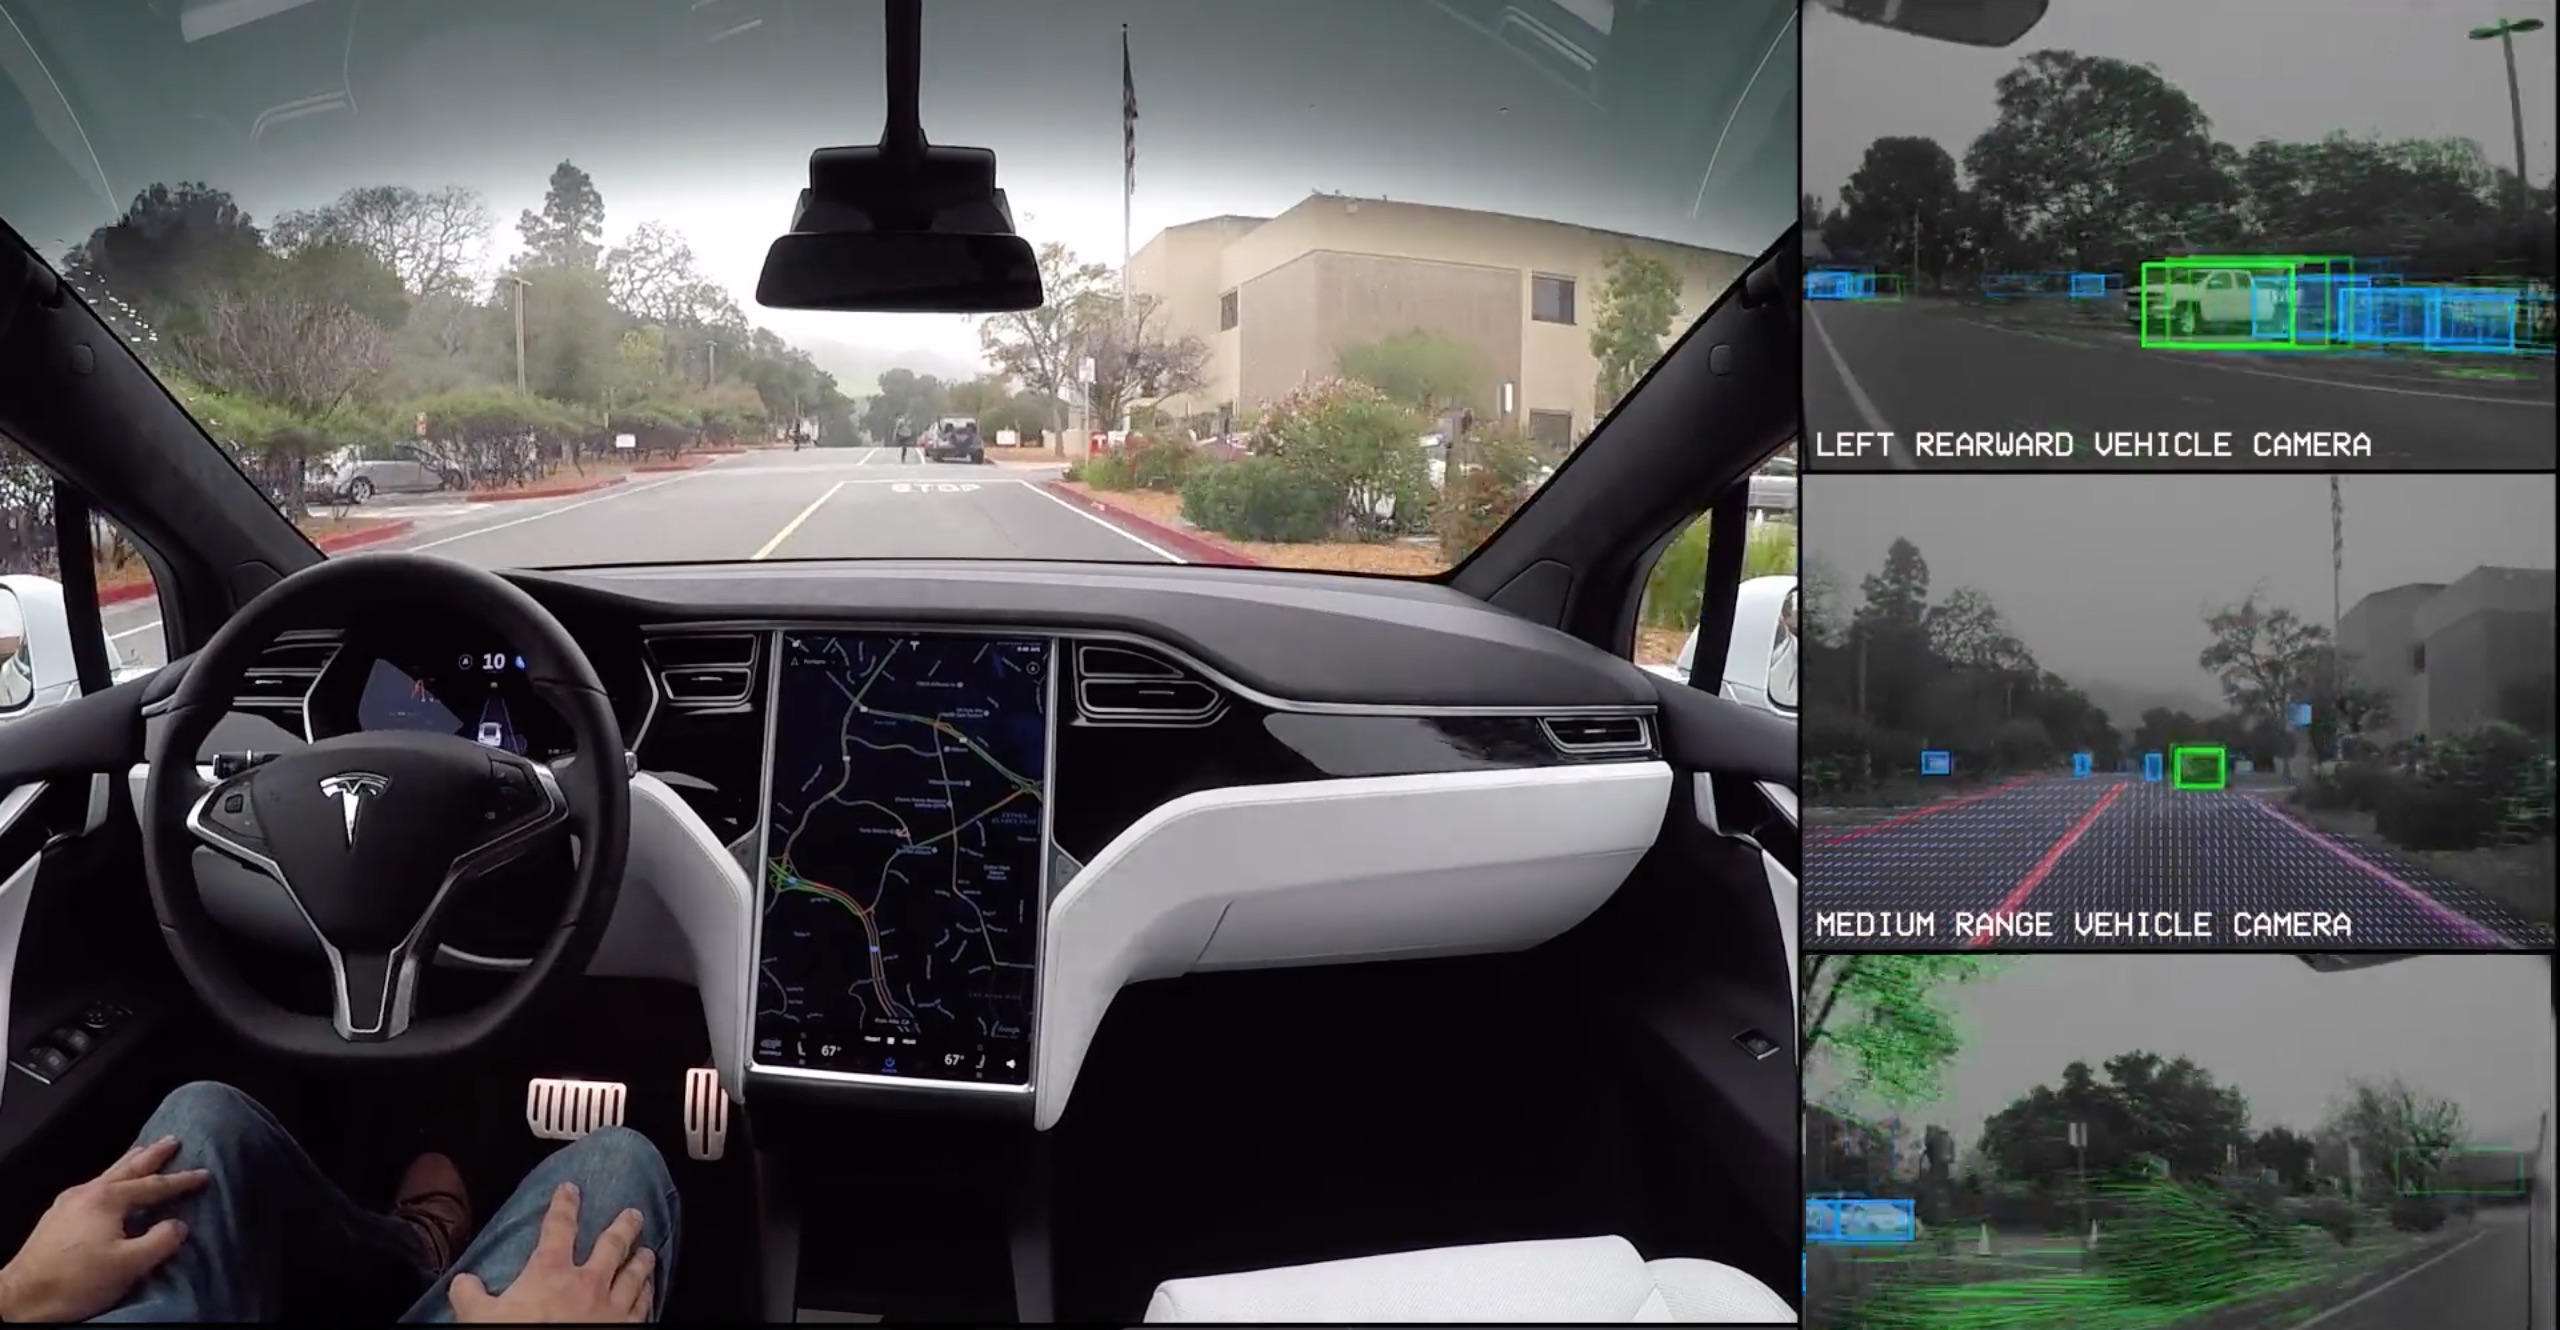
\includegraphics[width=\textwidth]{gfx/web/tesla-autopilot}\\
        Self-driving cars\\
        {\tiny Image: \href{https://www.tesla.com/}{https://www.tesla.com/}}\\
        {\tiny Movie: \url{https://www.youtube.com/watch?v=VG68SKoG7vE&t=166s}}
    \end{figure}
\end{frame}

\begin{frame}{Why Statistics?! Data-driven Modeling Applications}
    \begin{figure}
        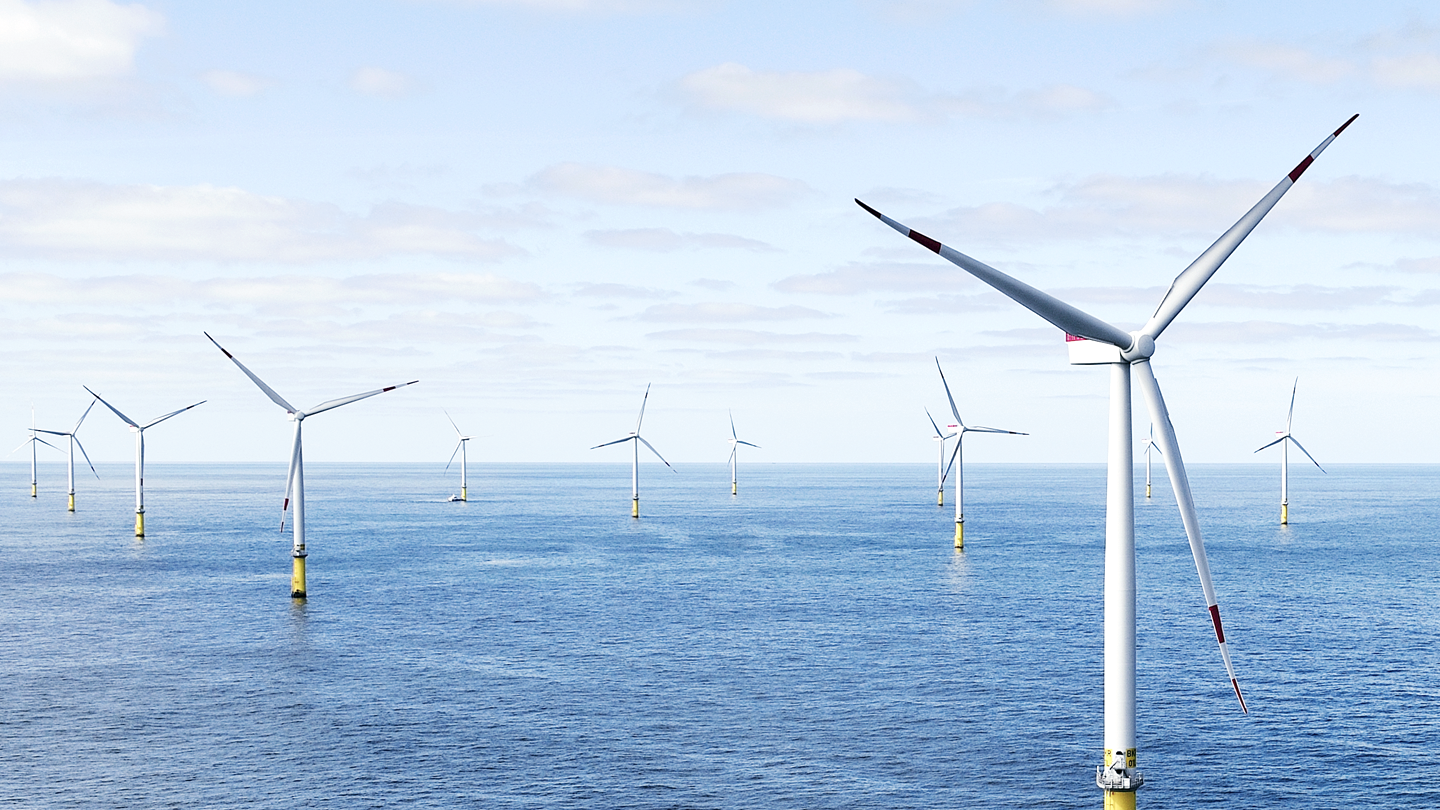
\includegraphics[width=0.9\textwidth]{gfx/web/wind-turbines}
        Predictive maintenance, e.g. of wind turbines\\
        {\tiny Image: \href{https://www.orsted.com/}{https://www.orsted.com/}}\\
        {\tiny Movie: \url{https://www.youtube.com/watch?v=BoFToRcfL0k}}
    \end{figure}
\end{frame}

\begin{frame}{Why Statistics?! Data-driven Modeling Applications}
    \begin{figure}
        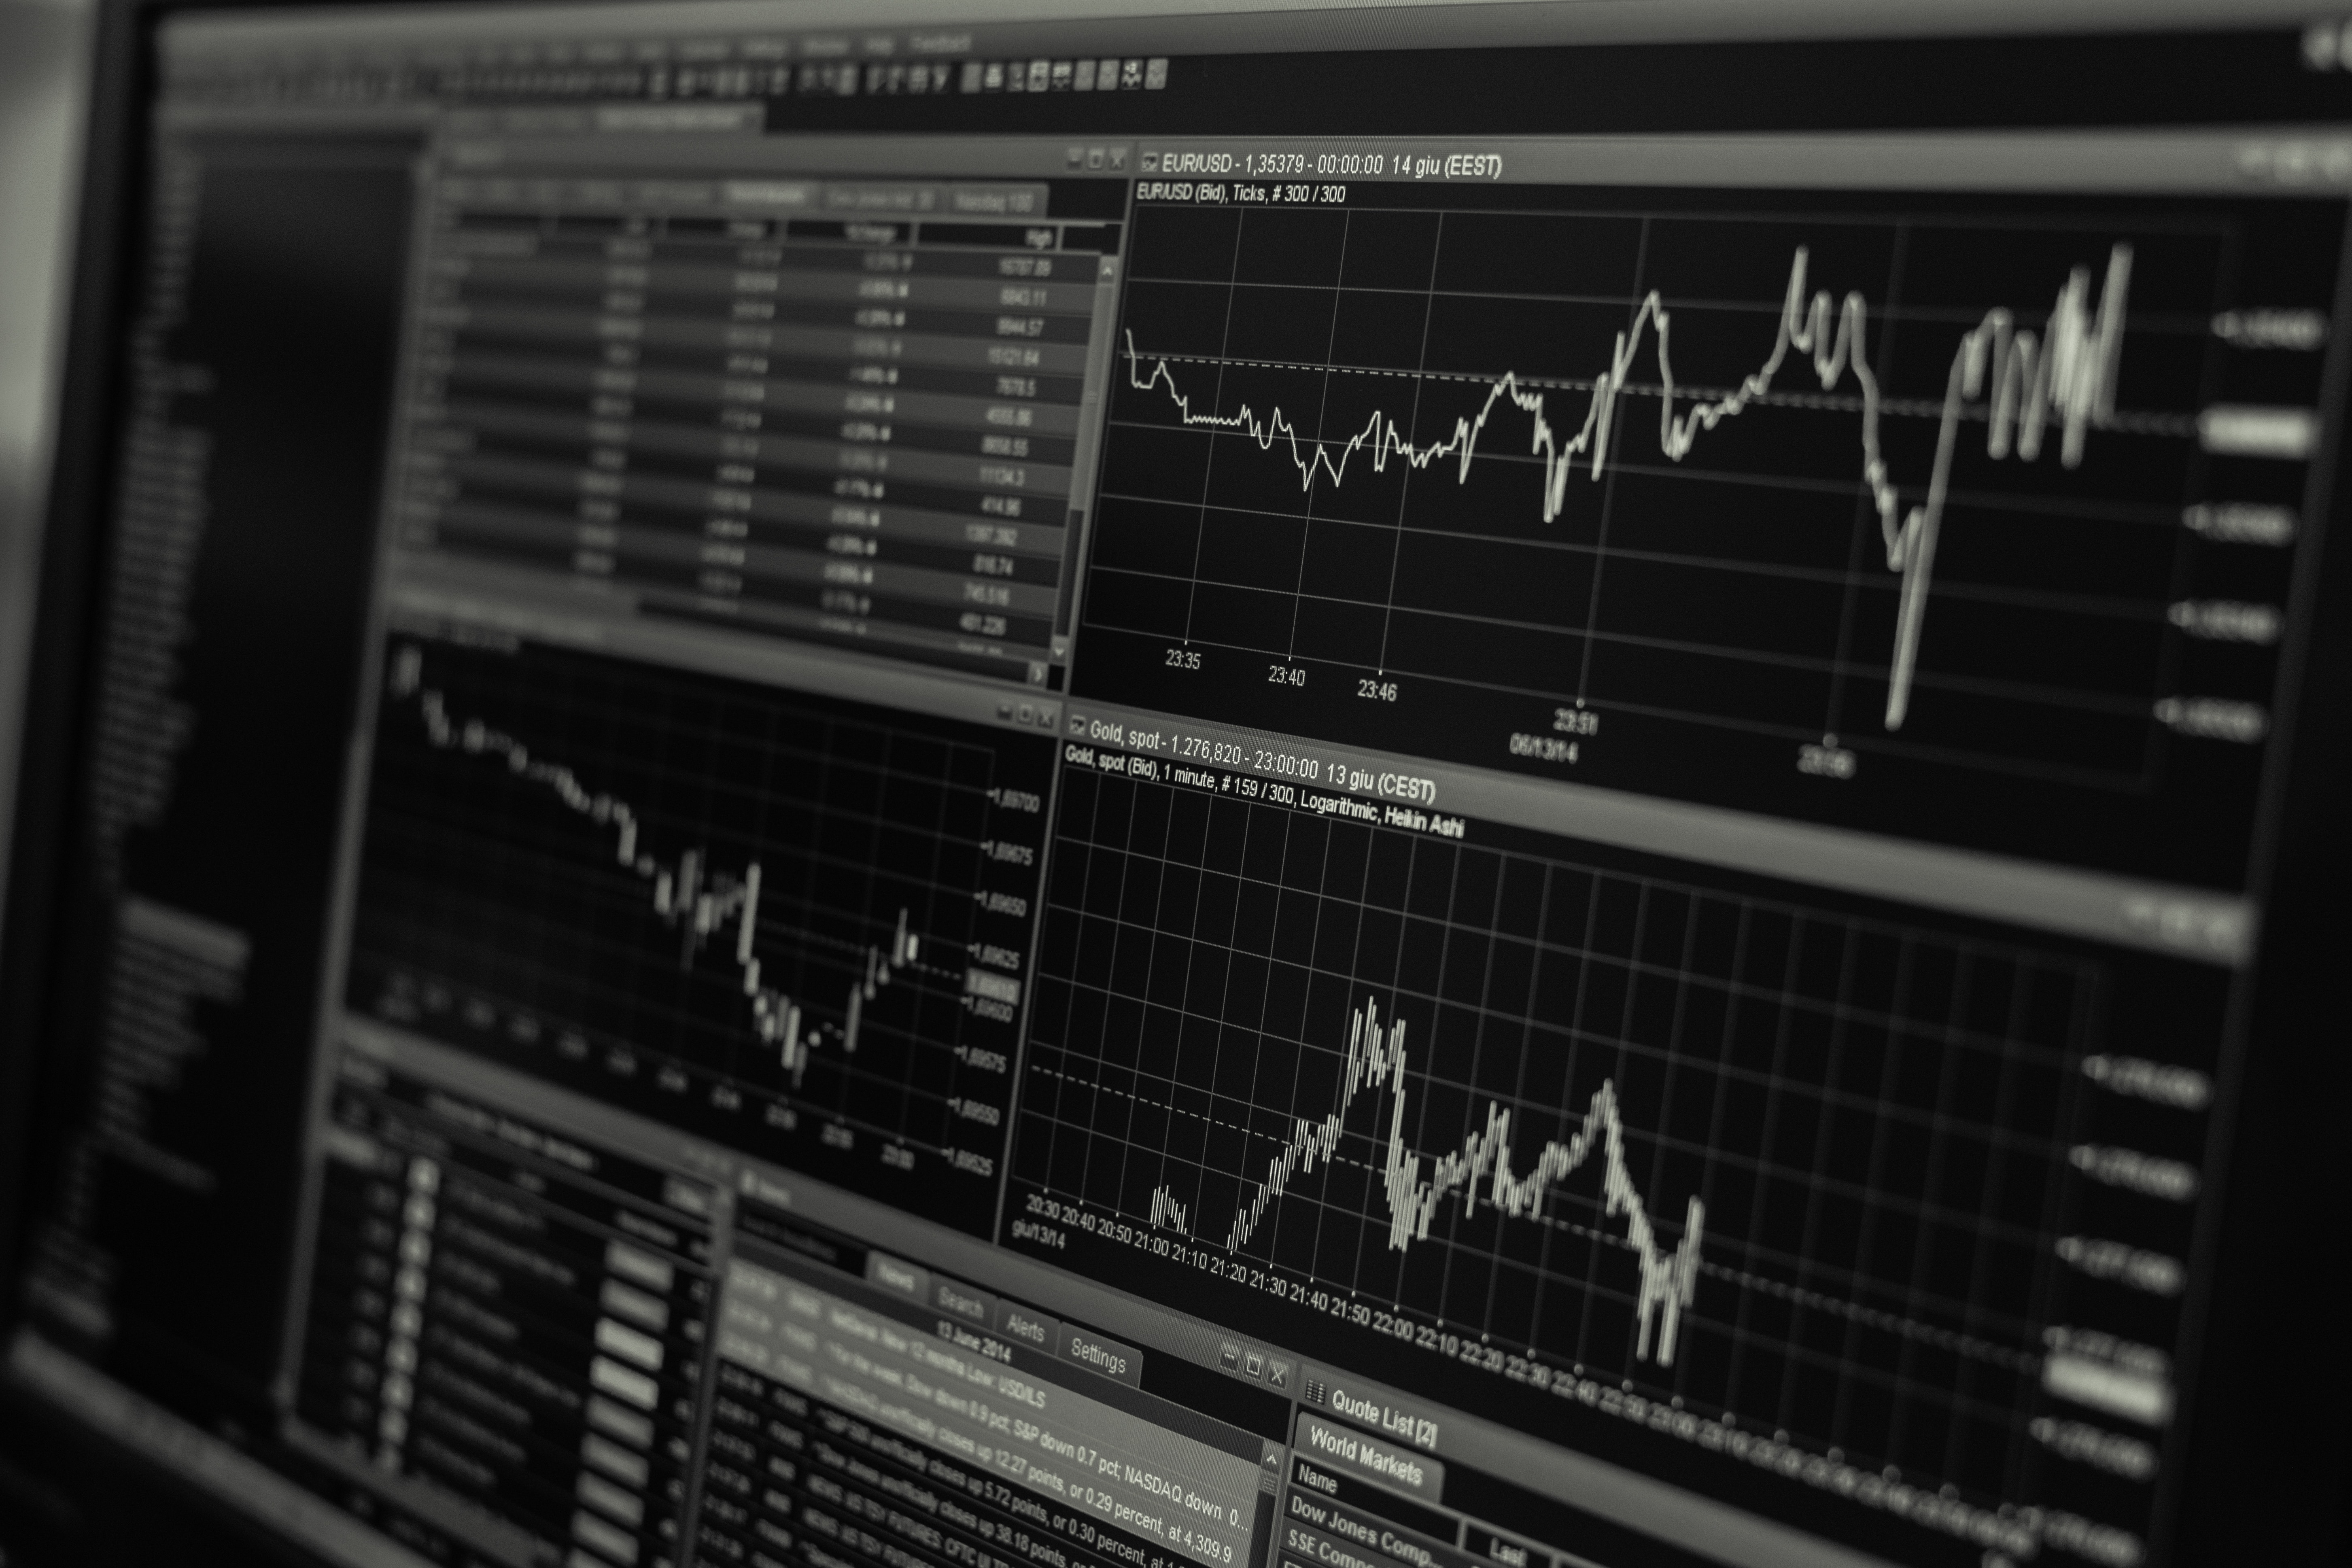
\includegraphics[width=0.9\textwidth]{gfx/web/black-and-white-business-chart}\\
        Algorithmic trading
    \end{figure}
\end{frame}

\begin{frame}{Why Statistics?! Data-driven Modeling Applications}
    \begin{columns}
    \begin{column}{0.5\linewidth}
        \includegraphics[width=\linewidth]{gfx/res1_zoom-eps-converted-to}
    \end{column}        
    \begin{column}{0.5\linewidth}
        \begin{itemize}
            \item OU44 building (SDU Odense)
            \item Thermal simulation
            \item Data-driven models (NN, NARX) outperformed physical models (R3C3, E+)
            \item \href{http://findresearcher.sdu.dk/portal/da/publications/comparative-analysis-of-white-gray-and-blackbox-models-for-thermal-simulation-of-indoor-environment-teaching-building-case-study(925c0fc9-7b0a-4689-a5bb-e6ec3a69f29b).html}{Click \emph{HERE} to go to the article}
        \end{itemize}
    \end{column}    
    \end{columns}
    
\end{frame}

\begin{frame}{Statistics vs. Domain Knowledge vs. Computer Science}
    \begin{figure}
    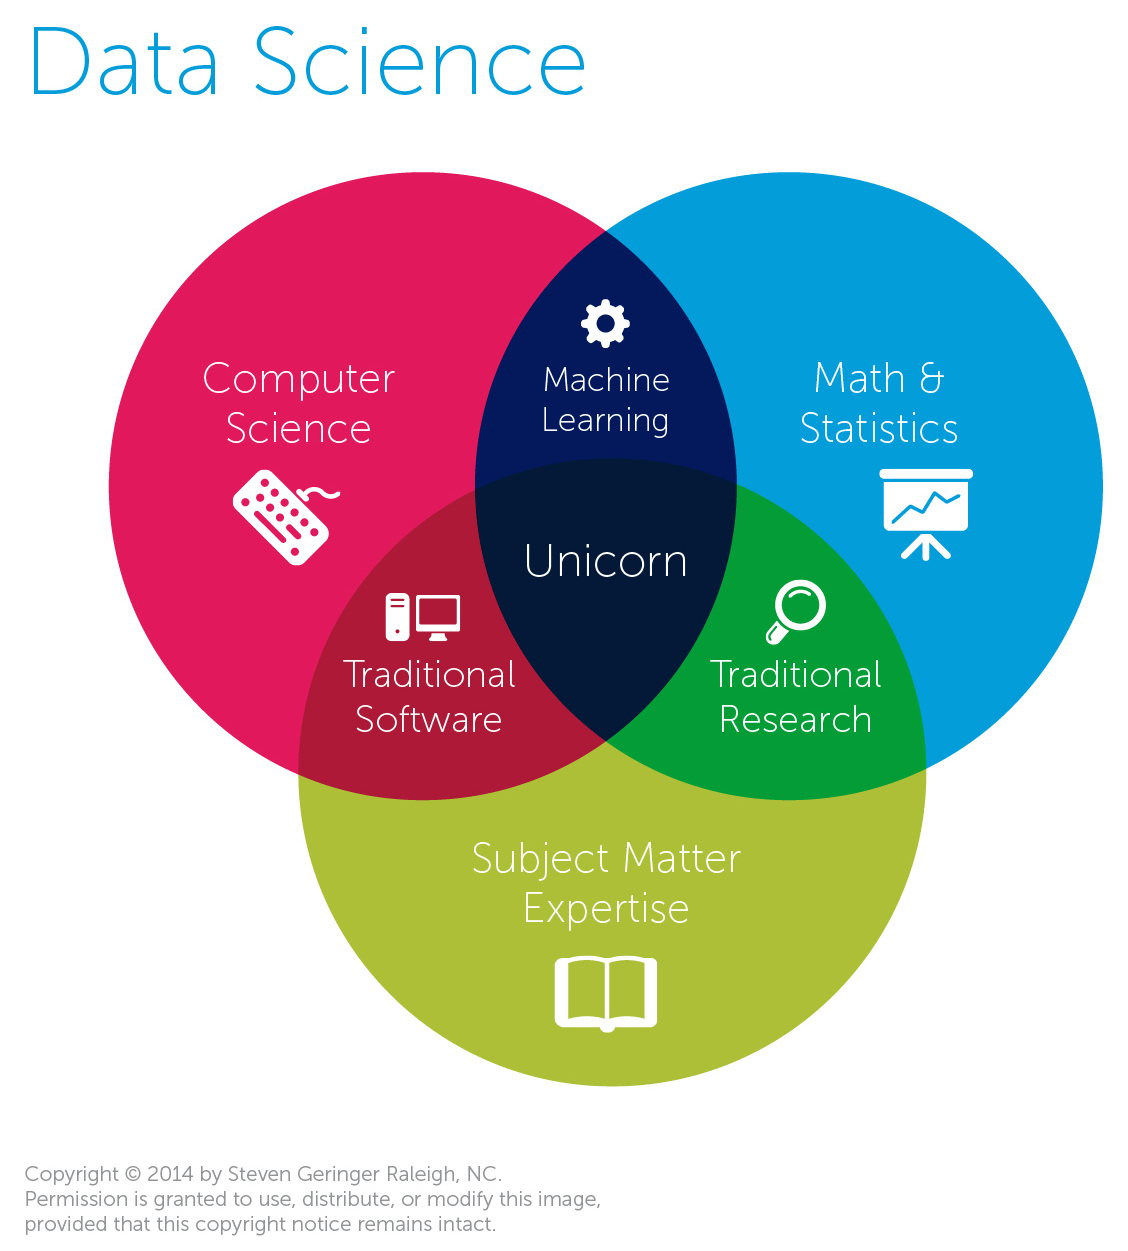
\includegraphics[width=0.65\textwidth]{gfx/web/data-science-venn-diagram}
    \end{figure}
\end{frame}

\begin{frame}{Job Market}
    41 offers in Denmark (6 February 2019):\\
    \url{https://www.jobindex.dk/jobsoegning?q=data-science}
    
    2875 offers in New York (6 February 2019):\\
    \url{https://www.indeed.com/q-Data-Scientist-l-New-York-jobs.html}
\end{frame}

\begin{frame}{Resources}
    This course is based on the following books and resources:
    \begin{enumerate}
        {\small
        
        \item \textit{OpenIntro Statistics},\\
        by D.M. Diez, C.D. Barr, M. Cetinkaya-Rundel,\\
        \url{https://www.openintro.org/}
        
        \item \textit{Introduction to Statistical Thought},\\
        by Michael Lavine,\\ \url{http://people.math.umass.edu/~lavine/Book/book.html}
    
        \item \textit{R for Data Science},\\
        by G. Grolemund and H. Wickham,\\
        \url{http://r4ds.had.co.nz/}
    
        \item \textit{The Introduction to Statistical Learning},\\
        by G. James, D. Witten, T. Hastie, R. Tibshirani,\\
        \url{https://www-bcf.usc.edu/~gareth/ISL}
    
        }
    
    \end{enumerate}
\end{frame}

\begin{frame}{Resources}
    Additional resources:
    \begin{enumerate}    
        \setcounter{enumi}{4}
        {\small
            
            \item \textit{Electronic Statistics Textbook},\\
            provided by StatSoft,\\
            \url{http://www.statsoft.com/Textbook}
            
            \item \textit{Experimental Design and Analysis},\\
            by H.J. Seltman,\\
            \url{http://www.stat.cmu.edu/~hseltman/309/Book/Book.pdf}
    
            \item \textit{Statistical Analysis with the General Linear Model},\\
            by Miller and Haden,\\
            \url{https://web.psy.otago.ac.nz/miller/StatsBook.htm}
                   
            \item \textit{The Elements of Statistical Learning},\\
            by T. Hastie, R. Tibshirani, J. Friedman,\\
            \url{https://web.stanford.edu/~hastie/ElemStatLearn}
            
            \item \textit{R Tutorial,}\\
            \url{https://www.tutorialspoint.com/r/index.htm} 
        }    
    \end{enumerate}
\end{frame}

\begin{frame}{Suggested Chapters}

    \begin{center}
    \begin{tabular}{l l}
        \hline
        Topic & References \\
        \hline
        Fundamentals                    & [1]:1 \\
        Probability                     & [1]:2 \\
        Distributions                   & [1]:3; [2]:1 \\
        Statistical Inference           & [1]:4,5 \\
        Simple Linear Regression        & [1]:7; [4]:3 \\
        Multiple Linear Regression      & [1]:7; [4]:3 \\
        Analysis of Variance            & [7]:2,3 \\
        R                               & [3]:1-21; [9]\\
    \end{tabular}
    \end{center}

\end{frame}

\begin{frame}{R}
    \begin{columns}
        \begin{column}{0.7\textwidth}
            About:
            \begin{itemize}
                \item R: \url{https://www.r-project.org}
                \item RStudio: \url{https://www.rstudio.com/}
            \end{itemize}

            Do the first steps:  
            \begin{itemize}
                \item Install RStudio
                \item Learn how to read docs
                \item Play around in the interactive mode
                \item Tutorial:\\ \url{https://www.tutorialspoint.com/r/index.htm}
            \end{itemize}
        \end{column}
        \begin{column}{0.3\textwidth}
            
\includegraphics[width=\linewidth]{gfx/web/Rlogo}
        \end{column}
    \end{columns}
\end{frame}

\begin{frame}{Why R?}
    
    \emph{R vs.\ other tools for data analysis:}\\
    \url{https://www.kdnuggets.com/2014/08/four-main-languages-analytics-data-mining-data-science.html}
    \vspace{7pt}
    
    \emph{R is:}
    \begin{itemize}
        \item easy to learn
        \item data- and statistics-oriented
        \item great at visualization ($\rightarrow$ show Shiny)
        \item open source!
    \end{itemize}

\end{frame}